% !TEX root = ../sel-report.tex
\section{What is a good requirement?}

\begin{mdframed}[outerlinewidth=0.5,roundcorner=5pt]
A requirement is a separately verifiable contractual statement
stating a need of the customer
\end{mdframed}

\begin{itemize}

\item The customer has certain needs and goals. However, those needs are likely to be vague or incomplete. If you build an actual product, it is hard to see how you (or your customer) would check that the product you built satisfies the customer's needs. What is needed is a \textbf{precise requirements document}.

\item A precise requirements document describes everything necessary to produce a safe and correct system---one that fulfills the needs of the customer---nothing more. 

\item The requirements document must provide the software developer with \textbf{all} the information needed for the system to be built.

\item At the same time the specification must not over-constrain developers by venturing into design and implementation detail.

\item The requirements document thus specifies \emph{what} the system will do---not \emph{how} the system will do it!

\end{itemize}

\section{System Under Description}

Some stuff. Here is a png figure (see folder ``pics'')

\begin{figure}[htb]
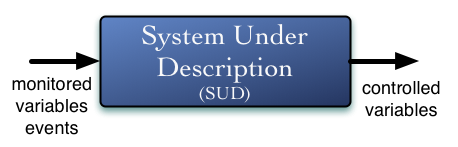
\includegraphics[width=.4\textwidth]{pics/sud.png}
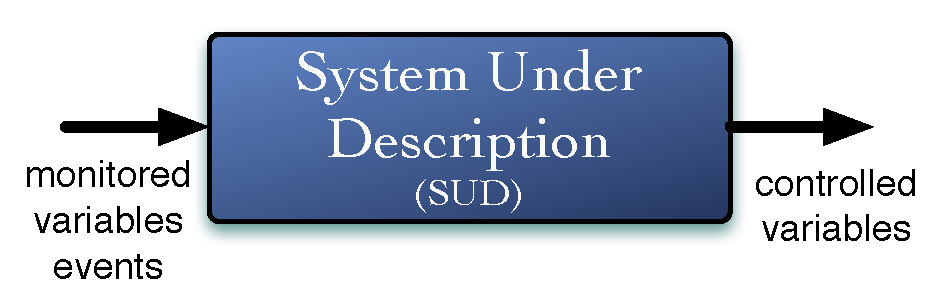
\includegraphics[width=.4\textwidth]{pics/sud.pdf}
\caption{PDF (right) displays better than jpeg or png (right)}
\label{fig:1}
\end{figure}

See Fig.~\ref{fig:1} for how to put an image in a figure environment. The ``htb'' says put the figure first here, then top of the page, then bottom, depending on layout algorithm. 

\section{R-descriptions and E-descriptions}
\reqm{ENV}
{Although it is physically possible for the trip and keypad commands to occur at the same time, the system is hardwired to respond sequentially (i.e. there is an arbitrary choice which one is dealt with first). Thus all signals arrive sequentially.}
{Refer to where your mathematical model uses this}
\label{E1}


\reqm{REQ}
{If the system is armed then a trip signal from the motion detector shall result in the siren being sounded.\\}
{Refer to mathematical model}
\label{R2}

\subsection{Subsection heading}

Other stuff with inline maths $p \limp q$ and 

\begin{equation}\label{eqn:1}
p \land q \lor r \limp z
\end{equation}

In (\ref{eqn:1}), we see how to write a formula.

Here is a verbatim environment with smaller text:

\begin{code}
=========================================
Use Case 1: uc1.txt: adding product types
=========================================
  report:      ok
  id:          0
  products:   
  stock:       
  orders:      
  carts:       
  order_state: 
->add_type("nuts")
  report:      ok
  id:          0
  products:    nuts
  ..
\end{code}

Here is some formatted PVS
\begin{pvs}
gate: THEORY
BEGIN
  p, q, r: bool
  not_gate(x: bool): bool = NOT x
  and_gate(x:bool, y:bool): bool = x AND y
  or_gate(x:bool, y:bool): bool = x OR y
  check1: CONJECTURE and_gate(p, not_gate(q)) => (p AND NOT q)
  check2: CONJECTURE and_gate(p, not_gate(q)) =  (p AND NOT q)

  circuit_implementation(x:bool, y:bool): bool = 
    and_gate(
              (or_gate(  and_gate(x, not_gate(y))
                       , and_gate(x,y))
             , y))

   and_conjecture: CONJECTURE
     and_gate(p,q) = circuit_implementation(p,q)

   or_conjecture:  CONJECTURE
     or_gate(p,q)  = circuit_implementation(p,q)
END gate
\end{pvs}

\begin{textbox}
Some text
\end{textbox}

\subsection{Signum Function}
Let's start with a simple example. In mathematics, the sign function or signum  (from \emph{signum}, Latin for ``sign") function $sgn(x)$ --- is a mathematical function that extracts the sign of a real number. In mathematical expressions the sign 

\begin{figure}[ht]
\begin{mdframed}[outerlinewidth=0.5,roundcorner=5pt]
\begin{minipage}{.4\textwidth}
\[sgn(x:\Rl) =
\begin{cases}
-1, &\text{if $x < 0$;}\\
0, &\text{if $x=0$;}\\
1, &\text{if $x >0$.}
\end{cases}\]
\end{minipage}
\qquad\qquad\qquad
\begin{minipage}{.5\textwidth}
\begin{tabular}{|l|l|}
\hline
        & $sgn(x)$ \\ \hline
$x < 0$ & -1     \\ \hline
$x = 0$ & 0      \\ \hline
$x > 0$ & 1      \\ \hline
\end{tabular}
\end{minipage}
\end{mdframed}
\caption{\small (a) Standard mathematical definition of $sgn(x)$. (b) Function table definition}
\end{figure}

The normal mathematical definition and the table layout are identical in meaning. However, the table layout is easier on the reader. Note that both description methods are \textbf{complete} and \textbf{disjoint}. 

\subsection*{Completeness}
The description of $sgn$ is complete because the function is defined for all possible inputs $x\in \Rl$. 

\subsection*{Disjointness}
The description is disjoint because each row in the table describes a case that is independent of the other rows --- hence avoiding inconsistencies 
--- where the same condition triggers different (and possibly contradictory) behaviours. 

For example, in a computer controlling a robot, we would not want the press of a \emph{move} button to signall to a robot to move right and move left at the same time.

The listing below shows how to describe the function in PVS.\footnote{%
See \url{https://wiki.eecs.yorku.ca/project/sel-students/p:tutorials:pvs:start}.}

 \section{Bibliography}
 
 See this \cite{Lamsweerde09}, this\ cite{GS93} and this \cite{Spivey92}. Run bibtex and then latex three times. 
\bibliographystyle{plain}
\bibliography{ref}